% chap1.tex - Week 1
\chapter{Week 1}
\section{Day 1 - ``Things need to change''}
\subsection{Meeting the Team}

If you're already a seasoned version control user, you may want to skip this chapter.
It's kind of like an introduction to why we even need version control systems in the first place.
This chapter looks at Tamagoyaki Inc's requirements and why they choose the VCS that seemed right for them.
Tamagoyaki Inc.
create software for turning a standard PC into a media center.
Their product ships to the end user and they rely very heavily on having a good presence at trade shows, in order to bring in sales.
The following conversation describes the events that led up to the defining "We need a VCS!" discussion.

\begin{trenches}
John sat at his desk and looked out of the window.
The rain was drizzling down the pane, but he didn't care.
It was a quiet Monday morning, the release had gone well on Friday and John was just thinking about implementing the new abstraction layer to the database he'd been asked for.
Through the music playing in his headphones he hardly noticed his boss, the chief designer and the CEO approaching his desk.

``John,'' shouted his boss, Markus, ``get your team into the board room. Now!''

Things didn't look good.

\thoughtbreak

``So, what we'd like to know John, is just how a bug that was supposed to have been\ldots'' the CEO back-tracked, ``that was demonstrated as being fixed two weeks ago, made it into the final release of the software?''

``I'm sorry,'' John started, before being cut off.

``Sorry doesn't cut it John,'' said the CEO, Wayne Tobi,
``This was almost a major embarrassment for Tamagoyaki Inc. We need to ensure this doesn't happen again. The demonstration at the trade show was close to a complete failure. Luckily someone had the good sense to bring a backup machine.''
He turned to Markus.
``I want a report on my desk by the end of the day that states what the problem was, how it slipped through our fingers and what safe guards we are going to put into place so that things like this never happen again.''

``Of course sir,'' Markus replied.
He was bright red with his own variety of embarrassment.

The room fell silent and a few minutes of silence passed before the meeting was drawn to a close and John and his team were allowed to leave.

\thoughtbreak

``So, you're telling me that when Simon came back from holiday, he picked up an older copy of the library from the network share and pushed his latest code into that?'' Markus was holding back the anger.

``It appears that way.'' Said John sullenly.

``Oh for crying out loud. How did this happen? Why wasn't he using the latest version? And why didn't QA pick up on it?'' Markus looked across the meeting room at John.
``John, you need to make sure this doesn't happen again. Find a solution!''
\end{trenches}

\subsection{The trouble with storage}

It's not like this situation is completely uncommon.
At one point or another most people have managed to pull old code from somewhere and mistakenly use it in place of the latest, up to date, version.
When storing code on network shares or on local disks, it's easy to lose sight of which version is which, no matter how good your naming convention is.
It's like trying to build one of the baked bean puzzles when you have three boxes of them and you tipped all the pieces into one box for simplicities sake.
Not so simple any more is it?

People have a tendency to use folder names which mean something to them.
However it doesn't necessarily follow that this name means something to another developer.
``Version 2.3 - fixed bug a'' only means something to you if you know what bug a is and something like ``Version 2.3 - fixed bug a(2)'' is even worse.
Unfortunately allowing people to free form type their own descriptive file names will always lead to problems like this.
When these files are stored on a network share, the problem is exacerbated ten fold because there is often no fixed reference point.

\index{Version Control}So what's the solution? Well, in a large number of cases version control can make sure that not only is there a defined place for data to sit, and with a defined structure, but also that you have a full history of the code.
Accountability is very important in code development, especially when releasing software to customers.
In some situations a customer will even mandate that the code being developed for them is stored in a version controlled environment.
In this way, the customer can ask when a certain piece of code was edited, or when an addition first entered the code base.

\section{Day 3 - ``A possible solution''}
\subsection{Version Control Nuances}

There are many offerings for version control out there, Git, Mercurial, Subversion, CVS, and Bazaar to name but a few of the open source ones.
Perhaps a more pertinent question is just which version control system to use.
Each of them has their relative advantages and disadvantages, but some will be suited to certain tasks more than others.
Also, it's worth noting that if you are interacting with other pieces of software, or share some development with another set of developers, it is a good idea to enquire to see what they are using.
Usually you'll find collaboration, forking and patching a lot easier if you're using the same version control system as your upstream or partners.

\begin{trenches}
``So really it seems like the only real solution to this problem bar Klaus' suggestions of reducing the workforce to only one developer, thank you Klaus,'' Klaus nodded in acknowledgement back to John, ``is to implement a version control system.''

Markus chewed his lip.
``I can see where you're coming from here John, but aren't version control systems really expensive?''

``There are a number of open source offerings we could take a look at first,'' piped up a new voice in the discussion, ``some of them are supposed to be pretty good.''

``Let's all go away, take a look at the various pros and cons and reconvene tomorrow to discuss the findings,'' said John.
``Sound fair?''
\end{trenches}

So now we need to take a look at some various features of version control systems and see what the various advantages and disadvantages are of each.
We are going to focus on Git here primarily, as this is what the rest of the book is all about.
It is assumed that if you are reading this book, you have most likely already made the decision about which version control system you are going to use.
So let's talk about the various features that are prevalent in most version control systems.

\index{Distributed Version Control}\subsection{Distributed Version Control}

Version control systems usually fit into one of two categories; centralised, or distributed.
Git is a distributed version control system.
It has been designed to run almost everything at a local level.
This will become much more clear when we talk about other features of Git a little later on, but for now just understand that Git isn't tied to a centralised repository.
This is super powerful.
No Really!

\index{Branching}\subsection{Branching}

Most version control systems offer branching as part of their default feature set.
Branching allows developers to create in essence a clone of their repository and mess around with it, safe in the knowledge that they can switch back to the original whenever they need to.
This allows developers the freedom to experiment with all manner of things without being afraid of affecting the original/clean code base.

Git implements branching in a special way.
Most older version control systems implement branching in a way that almost creates a separate copy of the repository.
This is slow and cumbersome.
Git's branching method gives developers the ability to create multiple local branches to play with.
Due to it's distributed nature, when pushing code to a more central location for others to pull from, developers can choose which branches they want to push, allowing code to be experimented with privately.

The implementation of branching in Git is fast.
Due to the fact that repositories are stored locally, the speed of creating a local branch is limited only by the speed of the disks on a local machine.

\index{Staging}\subsection{Staging}

Git deals with commits differently to most other version control systems by introducing the staging area.
The staging area allows developers to prepare their commits before they are written to the repository.
Why is this useful or any different to any other version control system.
In Git you can make a change to a file, add it to the staging area, and then continue to make changes to that file, even though you have not yet actually committed anything.
It should be noted that it's not absolutely necessary to use the staging area, but it is there for developers wishing to utilise it.

\index{workflow}\subsection{Workflow}

Due to the way that Git has been designed, it's possible to use it in practically any work flow you can think of.
Three of the most common workflows are explained below, and Git can work in any of these, making it one of the more versatile systems out there.

\index{workflow!Centralised}\subsubsection{Centralised Workflow}

In a centralised workflow, a single shared repository is used.
Multiple developers pull changes from here into local working copies, work on the local version, and then push it back up to the central location.

Git handles this workflow just like most other version control systems.
A developer can not push his changes until he has pulled everything up to the latest from the central repository and resolved any conflicts that may arise.

Using the centralised model for the workflow, each developer has the same level of access to the repository and is considered as \textbf{important} as each other.
For smaller teams, this method will work well, but as teams get larger, a centralised method may get tedious.
As more and more people start to access the same files, conflicts and other issues often begin appearing more often.

\begin{figure}[bt]
	\centering
	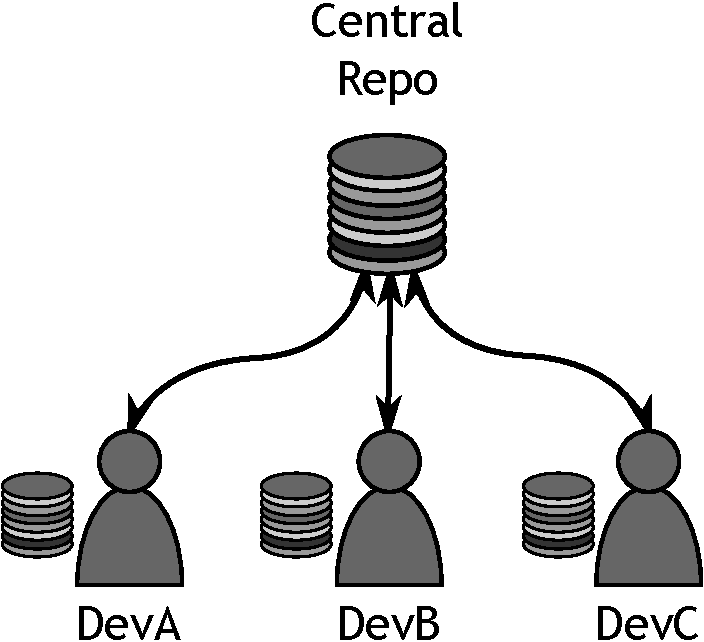
\includegraphics[width=7cm]{images/f-w1-d1.pdf}
	\caption{Centralised Workflow}
\end{figure}

\index{workflow!Integration Manager}\subsubsection{Integration Manager Workflow}
The integration manager workflow is similar to the centralised workflow because there is still a \textbf{blessed} repository which everyone uses as a reference.
The difference here is that there is only one person who has the rights to push changes to the \textbf{blessed} repository.
This person is referred to as the Integration Manager.

This workflow is handled exceedingly well by Git.
Developers will work on their repositories locally and then once they are happy, will push their changes to a location where the Integration Manager can see them.
The Integration Manager will then review the changes that the developers have made and will merge them into their own local repository.
Once they are happy that everything is working well, the Integration Manager will push their changes to the blessed repository so that all the other developers can access the changes.

\begin{figure}[bt]
	\centering
	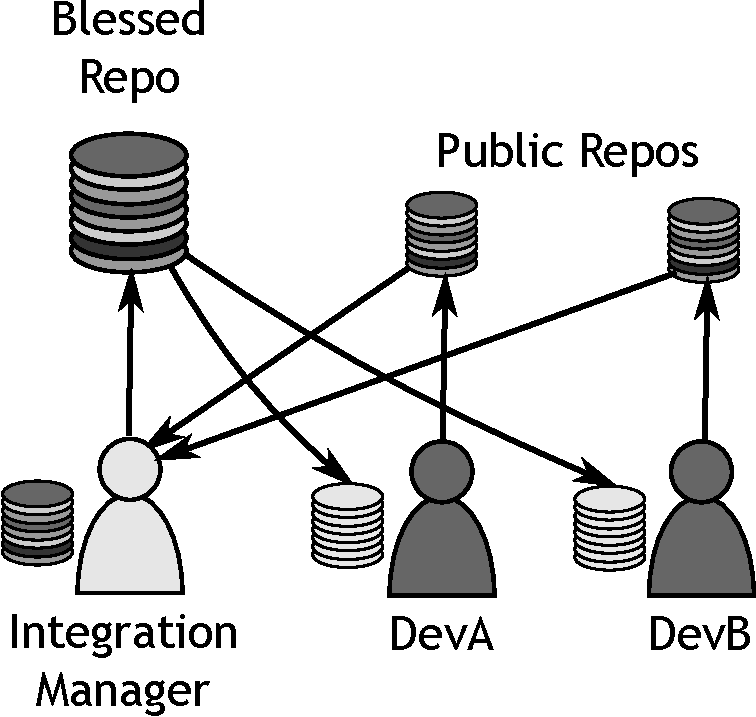
\includegraphics[width=7cm]{images/f-w1-d2.pdf}
	\caption{Integration Manager Workflow}
\end{figure}

\index{workflow!Dictator and Lieutenant}\subsubsection{Dictator and Lieutenant Workflow}

The dictator and lieutenant workflow is practically an extension to the integration manager workflow.
It is more suited to larger teams, where modules or sections of the code can be assigned to a \textbf{Lieutenant} who is responsible for blessing all of the changes to that particular section.

Once the Lieutenants are happy with their code, they make it available to the Dictator.
The Dictator then takes on a role similar to the Integration Manager from the previous model.
In the end, all of the changes are pushed to the blessed repository for the developers at the bottom of the tree to pull from.

\begin{figure}[bt]
	\centering
	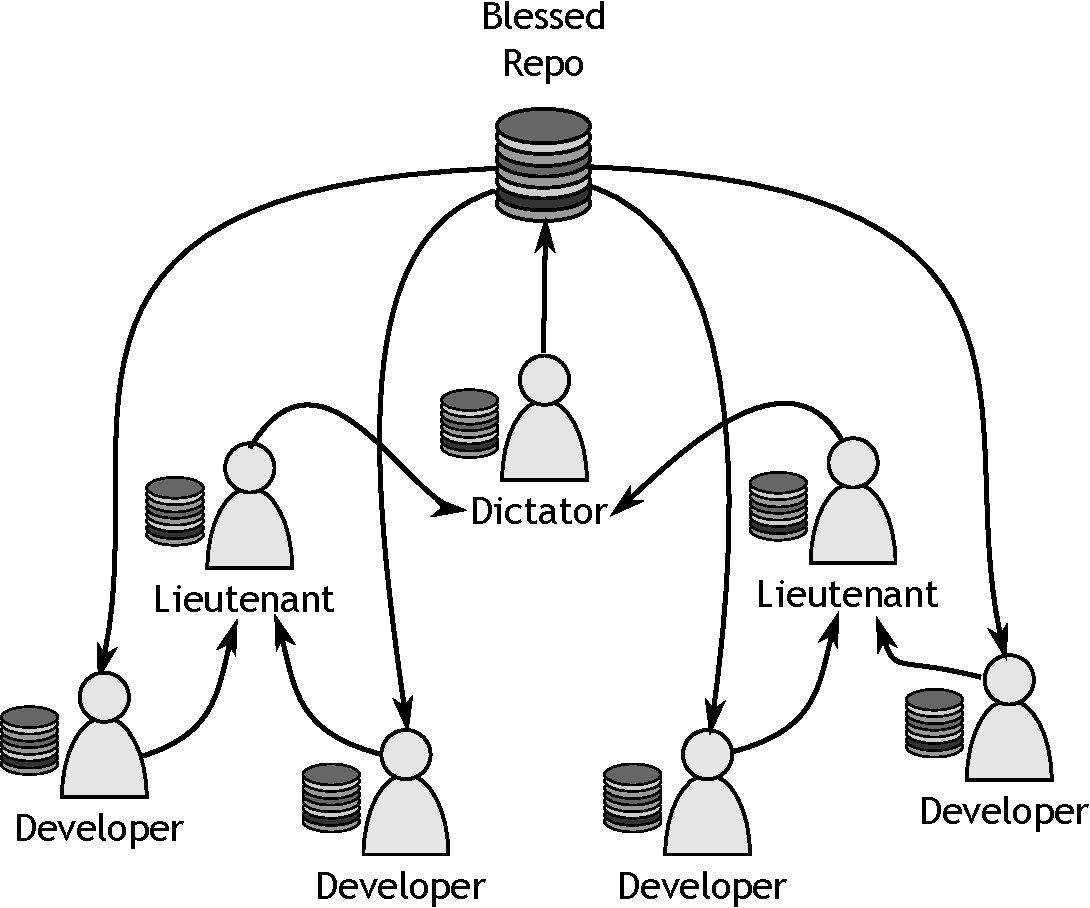
\includegraphics[width=7cm]{images/f-w1-d3.pdf}
	\caption{Dictator and Lieutenant Workflow}
\end{figure}

\begin{callout}{Terminology}{Blessed}\index{blessed (repository)}
A blessed, or canonical, repository is one which has the approval of the managers of the project.
The blessed repository is supposed to be the de facto standard where all other clones are made from.
If there is one place where code should be correct, it is the blessed repository.
If you are hosting the project in a public place, the blessed repository will usually be the one that is made available to people as a stable point for developing from.
\end{callout}

The main thing to remember, is that Git can utilise any of these workflows.
This makes it a very flexible system, allowing you to work in whichever way you decide.

\index{offline committing}\subsection{Offline Committing}

Perhaps one of the most useful and undervalued features of distributed version control systems is that of offline committing.
It may be undervalued because not all version control systems have it.
Offline committing is the ability to continue adding and committing files to the repository without being connected to a centralised repository.

When travelling or just simply when out of the office, developers and integrators alike are able to continue managing code, viewing histories, viewing diffs and committing changes to their repository.
This is all due to the fact that Git does 99\% of all of it's operations locally.
When a repository is cloned, Git actually sets up a copy of the entire repository locally, giving developers the flexibility to work anywhere, without requiring access to the company network.

When returning to the office, the developers simply push their changes to their ``public'' space, be it local or to a blessed location, and all of the commits that have been made whilst they are away are then made available to the rest of the team, including all history and snapshots.

\index{developer interaction}\subsection{Developer Interaction}

One factor to consider when choosing a version control system, is that of developer interaction.
By this we are referring to the way in which developers use and interact with the version control system itself.
There are four main methods for VCS interaction

\index{user interface}\index{user interface!GUI}\subsubsection{Graphical User Interface Client (GUI)}

A graphical user interface allows the developer, or user, to physically manipulate the repository using a mouse pointer and a graphically rich environment.
A GUI client will typically consist of separate application which is run when a user wants to make changes to a repository such as adding files or committing changes.

Some developers prefer having a separate client with which to interact with their repository, whilst others prefer to have things integrated a little more.

\index{user interface!shell extension}\subsubsection{Shell Extension Integration}

Shell integration allows the user to interact with their repository using the graphical environment that they would usually use for manipulating files and performing routine directory maintenance.
One of the most common Shell Extensions for Git is the TortoiseGit interface which integrates itself into Windows Explorer, allowing a user to right click on an entity whilst inside a git working tree, and be presented with a context sensitive menu for VCS operations.

\index{user interface!command line}\subsubsection{Command Line Interface (CLI)}

The command line interface is favour by many developers as they can script with it and can see exactly what is going on, often in much more detail that with a GUI.
The CLI gives total control over the product and it is worth noting that almost all version control systems start life as command line driven interfaces.
Why is this so? It can take a lot of time and effort to put all the options and nuances of a system into a GUI.
The CLI will almost always be the most powerful of all tools, especially where version control systems are concerned.

\section{Day 4 - ``A decision is reached''}

\subsection{Analysing Your Requirements}

The most important aspect of choosing a version control system, is to define your requirements.
These can be few, or they can be quite specific, let's see what John and his team decide are the most important aspects for them and ultimately what they decide upon.

\begin{trenches}
``Offline committing seems like it's a pretty useful thing to have.'' Mike said nodding.
``Especially with people like John travelling all the time.''

``I have to admit, it would be nice to be on the plane, and be able to pull all the code together, knowing all of the history of each section,'' replied John.
``The branching in Git seems to be quite powerful as well.''

``I must admit,'' chimed in Klaus, ``I've used branching a bit in Subversion before and it was a lifesaver.
It's supposed to be super fast in Git too.''

``And owing to the fact that Git seems to support several workflows, it means we can try them out and see how they work for us.'' Markus looked at the team.
``Are we settled on Git then?''

The team nodded and everyone walked out of the board room except John.
Things were about to get interesting for him.
Very interesting.
\end{trenches}

Since this book is all about Git, we won't delve too far into the workings or features of other version control systems.
Hopefully, this chapter has given you enough information to go and check out some of the other systems, if you feel the need to.
The main thing to bear in mind is that Git is a Distributed Version Control system.
While this is so, it is equally important to remember that it can be used in the same workflow models as Centralised Version Control systems.

John and his teams requirements are nothing special.
They are a smallish team looking to reap the benefits of having their code in a well organised system.
They are also looking to reorder their team functions and dynamics in order to fit around the version control system and really make it core to their development.

Version control is not a replacement for workflow.
It is not intended to make everything better.
If you have people going off and doing their own thing and being careless about the way they work, version control is not going to suddenly fix everything.
A tool is just that, a tool and version control is no different.
You can buy the messiest builder in the trade a nice shiny new tool box, but unless they have the mindset to want to change, you'll probably find that all the tools end up in the largest compartment at the bottom.

\section{Day 5 - ``Working like a team''}

\index{team organisation}\subsection{Team Organisation}

Now that we have the basics dealt with, let's take a little look at how John arranges his team, and see whether version control is going to work for them.
It is important that the team understands how the model should work, what they are expected to do and what level of access they have.
Most of the time people will get more frustrated about not know what they should or shouldn't be doing, rather than that they do or don't have access to certain things.

\begin{trenches}
It was 4:36pm on the Friday and the table in the board room was littered with empty coke cans, pizza boxes and one Japanese bento lunchbox, owned by a particularly stubborn member of the team who had vowed never to eat pizza again.
It had been Marcus' idea to bring in the food reinforcement to help the discussions along.
The team were trying to decide how to organise their model.

``There's nothing to say we can't use a combination of the models is there?'' asked Mike.

``I suppose not,'' said John.
``What did you have in mind.'' His glasses were slipping down his forehead now and he was getting pretty tired.

``Well, I figure, we basically have the software split into two parts. We have the library, which myself, Klaus and Jack work on. Then there's the UI elements which Simon, Martha and Rob handle. I know there are the tools which Eugene works on too.''
Everyone had started to listen to Mike as he continued.
``John, you don't want to have to deal with the library component as this more Klaus' space. So why don't we have two dictators. Klaus and yourself have access to push up to the blessed repository. John can pull from his guys, Klaus from his and we end up with an good model for version control.''

John raised his eyebrows, ``Not bad Mike,'' he said, genuinely impressed.
After spending a few hours going through the various models and who was in charge of what, it felt good to have finally reached a decision.

``So, we start on Monday then?'' asked Markus, who had been listening from the other end of the table.

``Indeed.'' Announced Klaus, ``Monday we all become Gits!''
\end{trenches}
